\chapter{Experimenty DOSIS a DOSIS 3D}
Informace v této kapitole byly čerpány převážně ze zdrojů \cite{dosis,dosis2}.

Experiment DOSIS (Dose Distribution Inside the ISS, distribuce dávky uvnitř ISS) probíhal v letech 2009-2011, experiment DOSIS3D probíhá od roku 2012. Jejich cílem je stanovení prostorové distribuce dávky v modulu ISS Columbus a získání dat, která by vedla k vytvoření 3D modelu rozložení dávek/dávkového ekvivalentu.
%a DOSIS 3D probíhají roku 2009 za účelem vyšetření prostorové distribuce dávky v modulu ISS Columbus. Kýženým cílem bylo získání dat, která by vedla k vytvoření 3D modelu této distribuce.

Na experimentech se podílí řada institucí z různých zemí, jejich přehled je v tab.~\ref{tab:dosis_instituce}. Hlavním koordinátorem je DLR. 
\begin{table}[H]
  \centering
\renewcommand{\baselinestretch}{0.8}
\renewcommand{\arraystretch}{2}
\footnotesize
\caption{Organizace podílející se na experimentech DOSIS a DOSIS3D. \cite{dosis}}
  \label{tab:dosis_instituce}
  \begin{tabularx}{\textwidth}{X}
	\toprule
German Aerospace Center (DLR), Institute of Aerospace Medicine, Linder Höhe, 51147 Köln, Germany\\
Christian Albrechts Universität zu Kiel (CAU), Christian-Albrechts-Platz, 24118 Kiel, Germany                                    \\
Institute of Nuclear Physics, Polish Academy of Sciences (IFJ), PL-31342 Krakow, Poland                                          \\
International Atomic Energy Agency (IAEA), Division of Radiation, Transport and Waste Safety, 1400 Vienna, Austria               \\
Technische Universität Wien, Atominstitut (ATI), Stadionallee 2, 1020 Vienna, Austria                                            \\
EGB MedAustron, Marie-Curie-Straße 5, 2700 Wiener Neustadt, Austria                                                              \\
Centre for Energy Research, (MTA EK/AERI), Konkoly Thege ut 29-33, 1121 Budapest, Hungary                                             \\
Nuclear Physics Institute of the CAS (NPI), Department of Radiation Dosimetry, Na Truhlarce 39/64, 180 00 Prague, Czech Republic \\
Belgian Nuclear Research Center (SCK$\cdot$CEN), Boeretang 200, 2400 Mol, Belgium    \\
NASA, Space Radiation Analysis Group (NASA/SRAG), Houston, TX 77058, USA       \\
Leidos, Exploration \& Mission Support, 2400 NASA Pkwy, Houston, TX 77058, USA  \\
Physics Department, Oklahoma State University (OSU), Stillwater, OK 74078, USA \\
National Institute of Radiological Sciences (NIRS), National Institutes for Quantum and Radiological Science and Technology (QST), 4-9-1 Anagawa, Inage, 263-8555 Chiba, Japan\\
OHB System AG, Universitätsallee 27-29, 28359 Bremen, Germany\\
\bottomrule
  \end{tabularx}
\end{table}

Měření byla, respektive jsou prováděna pasivními a aktivními detektory, které jsou pevně umístěny v modulu Columbus. Pasivní detektory zajišťují určení prostorové distribuce dávky a dlouhodobého vývoje pole záření, aktivní naopak slouží k určení změn pole záření v čase. V případě aktivních detektorů se jedná o dva detektory DOSTEL (DOSimetry TELescope). V dalším textu se budeme zabývat pouze pasivními detektory.

\section{Rozmístění pasivních detektorů}
V rámci experimentu DOSIS, resp. DOSIS3D je v modulu Columbus rozmístěno jedenáct PDP (Passive Detector Packages, balíčky pasivních detektorů), které obsahují termoluminiscenční detektory (TLD), detektory využívající optickou stimulaci (OSLD) a detektory stop v pevné fázi (TED). Na obr. \ref{fig:columbus_rozmisteni} vidíme rozmístění PDP; pět z nich je umístěno na čelní stěně, dalších šest na zadní stěně. Jedenáctý balíček označený symbolem X, též označovaný jako Triple PDP (trojitý PDP), je umístěn blízko aktivních detektorů a pokrývá větší plochu než ostatní PDP. Osm PDP je umístěno ve skříňových modulech (viz oddíl \ref{sec:ISS_columbus}); více informací o umístění pasivních detektorů je k dostání v \cite{dosis}. %další obrázek???
\begin{figure}[ht]
  \centering
  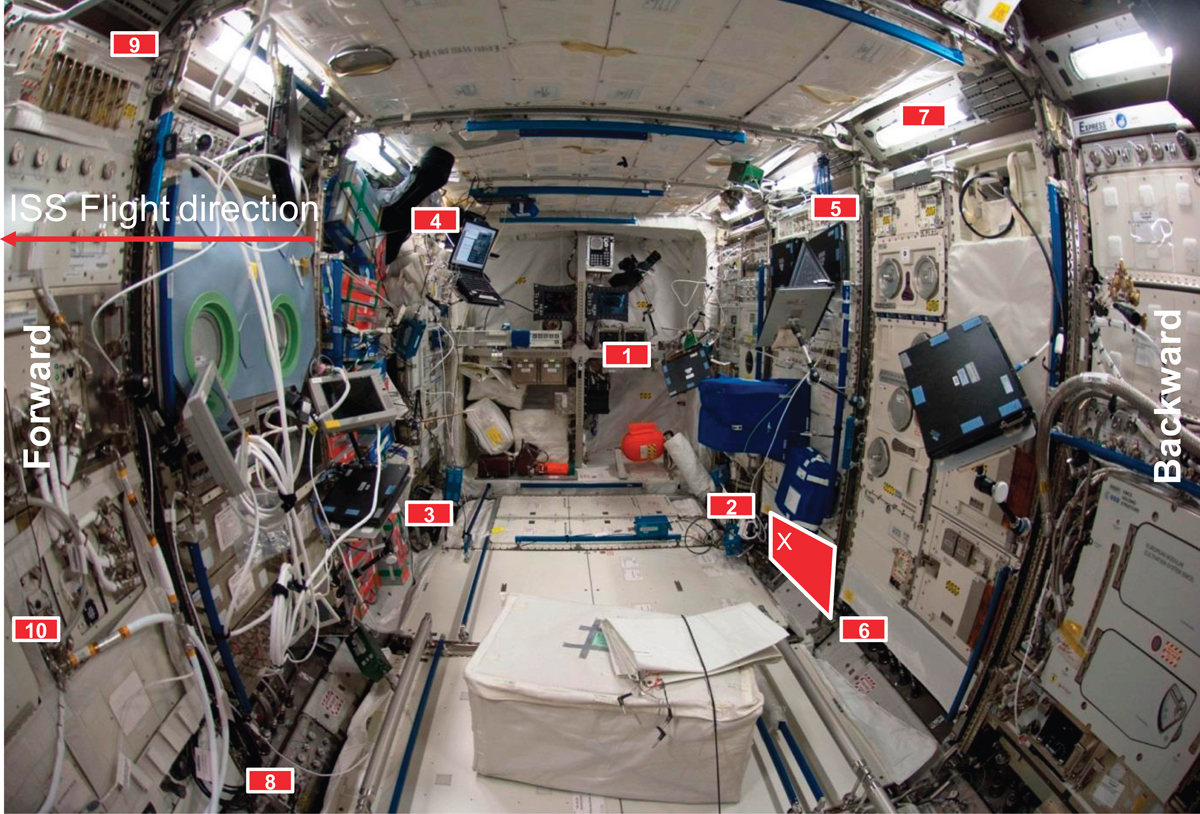
\includegraphics[width=\textwidth]{columbus_rozmisteni.jpg}
  \caption{Rozmístění jedenácti balíčků s pasivními detektory v modulu Columbus; jedenáctý je označen symbolem X a v jeho blízkosti jsou umístěny i aktivní detektory. Obrázek dále obsahuje šipku ukazující směr letu. \cite{dosis}}
  \label{fig:columbus_rozmisteni}
\end{figure}

\section{Průběh experimentů}%mozna DOPLNIT:DOSTEL-1 meril kratsi dobu nez DOSTEL-2!!!!!!!!!!!!!
Experiment DOSIS probíhal mezi lety 2009 a 2011. Doba trvání experimentu DOSIS3D byla původně stanovena na rozmezí let 2012-2016, avšak v roce 2016 byla prodloužena a experiment stále běží. V rámci těchto experimentů bylo v modulu Columbus zatím k dnešnímu datu (13. 5. 2017) postupně upevněno 10 sad pasivních detektorů (DOSIS -- dvě sady, DOSIS3D -- devět sad) a na květen/červen 2017 se plánuje upevnění jedenácté. Každá sada obsahovala výše zmíněných 11 PDP. Tab.~\ref{tab:dosis_timeline_passive} obsahuje informace o obměně sad pasivních detektorů (dopravení na ISS, instalaci, doba používání, ukončení měření,
návrat na Zem, nadmořská výška ISS); u sad 7, 8, 9 experimentu DOSIS3D nejsou doposud k dispozici údaje o nadmořské výšce; sada 10 je stále na ISS. 

První z experimentů započal 15. července 2009 startem raketoplánu Endeavor, na jehož palubě byla
první sada pasivních detektorů spolu s aktivními detektory \mbox{DOSTEL-1,2}. Jeho část skládající se z měření pasivními detektory skončila 26. května 2010 návratem druhé sady. Experiment DOSIS3D započal 15. května 2012 startem lodi Soyuz 30S. 
\begin{table}[ht]
  \centering
\footnotesize
  \caption{Časový vývoj používaných sad pasivních detektorů. Tabulka dále obsahuje dobu, kterou daná sada strávila na misi (tj. od startu do návratu na Zem), v závorce je doba, po kterou pasivní detektory byly umístěny v dané pozici/místě; pokrytí je podíl těchto dvou dob. Poslední sloupec obsahuje rozmezí nadmořské výšky, ve které se ISS v daný časový úsek nacházela~\cite{dosis}. U sad 7,8,9 nejsou dosud k dispozici informace o nadmořské výšce. Na ISS se nyní nachází 10. sada experimentu DOSIS3D.}
  \label{tab:dosis_timeline_passive}
  \begin{tabularx}{\textwidth}{llllll}
	\toprule
	&Sada&	Počátek-konec	&Doba trvání [dny]	&Pokrytí [\%]	&Nadmořská výška ISS [km]\\
	\midrule
DOSIS	&1	&Červenec 2009-	&136 (127)	&93,3	&339-348\\
		&	&Listopad 2009	&		    &       &       \\
		&2	&Listopad 2009-	&191 (178)	&93,2	&337-349\\
		&	&Květen 2010	&		    &       &       \\
DOSIS3D	&1	&Květen 2012-	&125 (113)	&90,4	&397-417\\
		&	&Září 2012		&	        &       &       \\
		&2	&Říjen 2012-	&144 (137)	&95,1	&407-416\\
		&	&Březen 2013	&		    &       &       \\
		&3	&Březen 2013-	&167 (156)	&93,4	&407-416\\
		&	&Září 2013		&	        &       &       \\
		&4	&Září 2013-		&167 (156)	&93,4	&413-418\\
		&	&Březen 2014	&		    &       &       \\
		&5	&Březen 2014-	&170 (161)	&94,4	&407-416\\
		&	&Září 2014		&	        &       &       \\
		&6	&Září 2014-		&167 (161)	&96,4	&413-418\\
		&	&Březen 2015	&			&		&		\\
		&7	&Březen 2015-	&259 (256	&98,8	&		\\
		&	&Prosinec 2015	&			&		&		\\
		&8	&Prosinec 2015- &186 (180)	&96,8	&		\\
		&	&Červen 2016	&			&		&		\\
		&9	&Červenec 2016	&115 (109)	&94,8	&		\\
		&	&Říjen 2016		&			&		&		\\
		\bottomrule
  \end{tabularx}
  %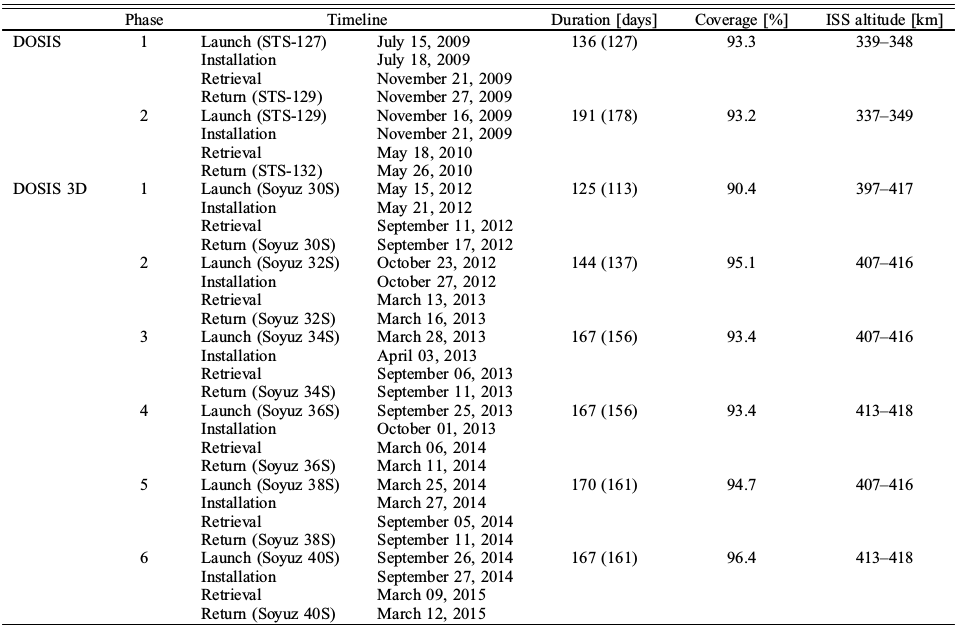
\includegraphics[width=\textwidth]{dosis_timeline_passive}
\end{table}
\subsection{Vývoj nadmořské výšky a slunečního cyklu}\label{sec:dosis_altitudeSlunecniCyklus} %špatné odsazení
Naměřené dávky a dávkové ekvivalenty jsou ovlivněny řadou parametrů. Nadmořská výška a fáze slunečního cyklu jsou jedny z nejvýznamnějších. 

Na obr. \ref{subfig:dosis_altitude} je znázorněn časový vývoj nadmořské výšky ISS. Pro DOSIS nadmořská výška nabývala hodnot z intervalu [337, 375] km, pro DOSIS3D nabývala hodnot z intervalu [398, 417] km. V obrázku lze vypozorovat prudký nárůst z cca 340 km do 375 km, který se udál ke konci experimentu DOSIS; tehdy již měřily pouze aktivní detektory. Změna nadmořské výšky ovlivňuje ozáření stanice (viz oddíl \ref{sec:kosmickeZareni_altitude}). 

Z informací v oddílu \ref{sec:kosmickeZareni_solar} plyne, že za slunečního maxima je obdržená dávka od GCR nejmenší a naopak za slunečního minima největší (za předpokladu stálosti ostatních parametrů ovlivňujících velikost obdržené dávky). To je znázorněno na obr. \ref{subfig:dosis_solarCycle}, kde je zobrazena závislost četnosti detekovaných neutronů na čase (počet detekovaných neutronů klesá s rostoucí sluneční aktivitou). Experiment DOSIS probíhal za slunečního minima (2009 až 2011) a naopak experiment DOSIS3D probíhal za slunečního maxima, které nastalo v letech 2013 a 2014.   
\begin{figure}[h]
  \centering
  \begin{subfigure}{0.45\textwidth}
	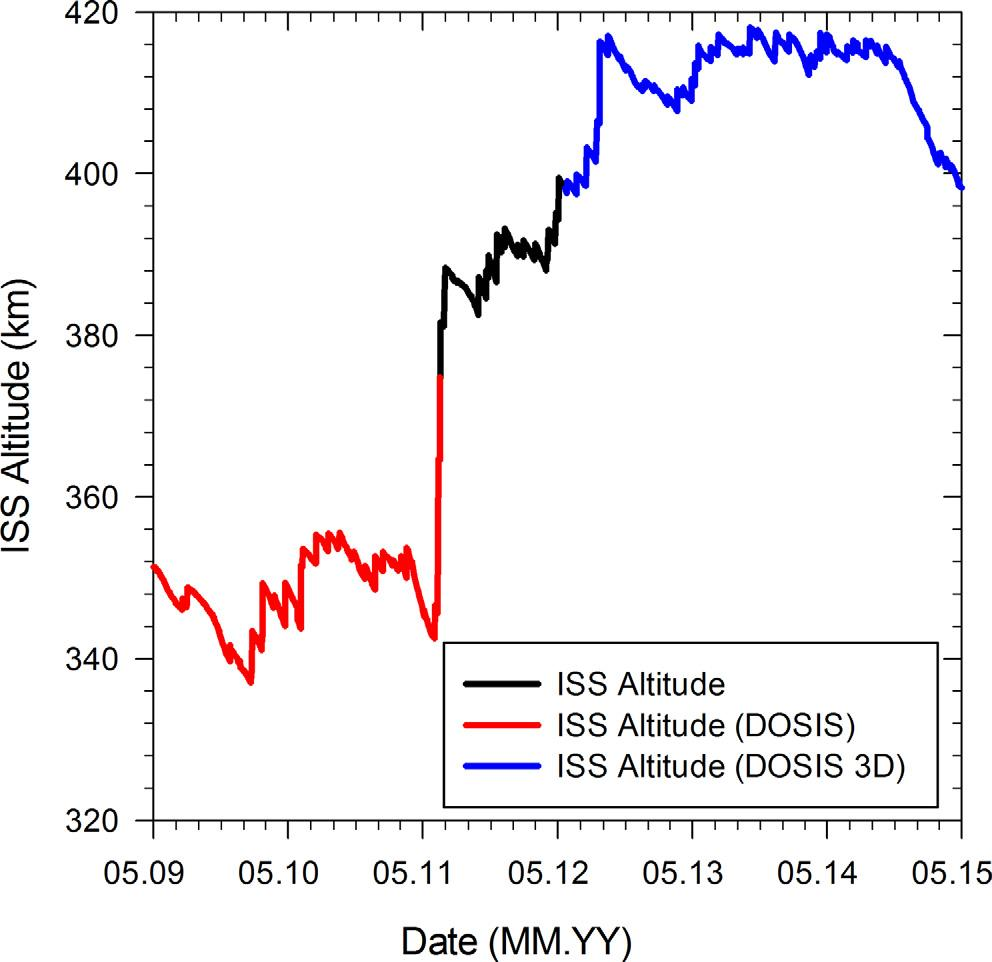
\includegraphics[width=\textwidth]{dosis_altitude.jpeg}
	\caption{}
	\label{subfig:dosis_altitude}
  \end{subfigure}
  \begin{subfigure}{0.45\textwidth}
	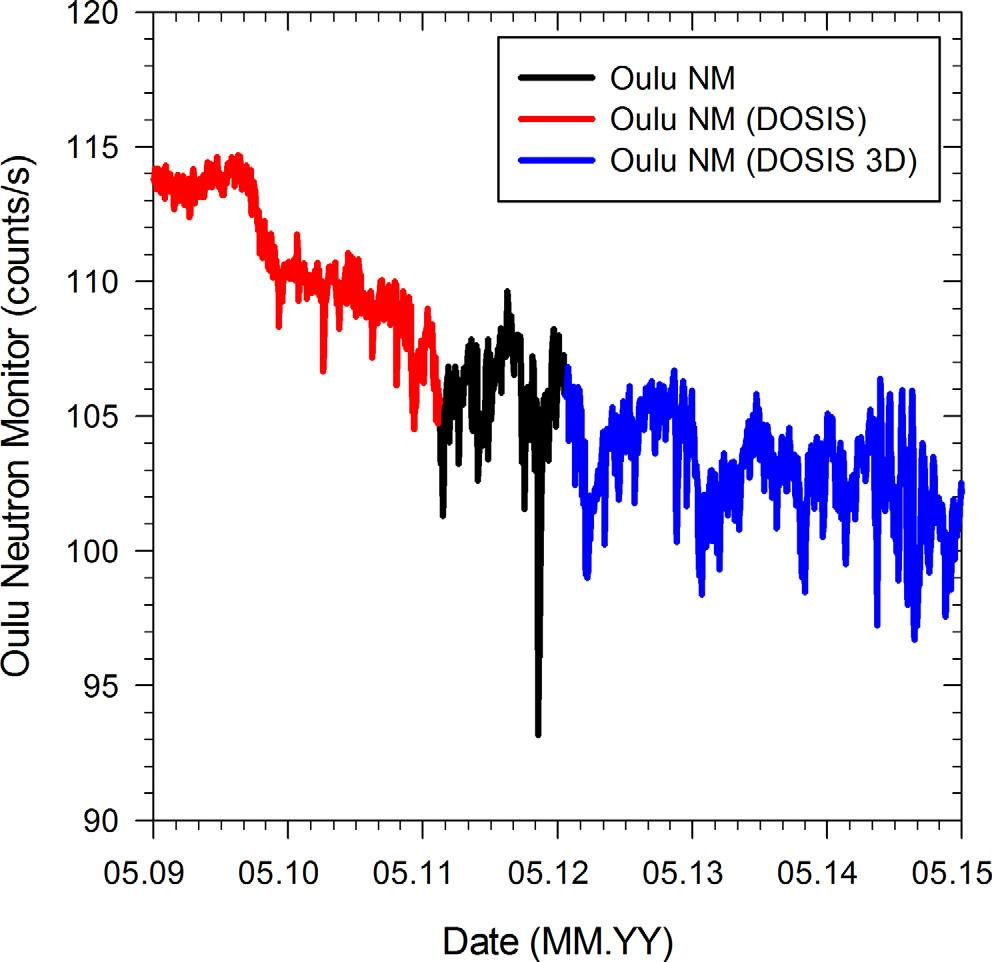
\includegraphics[width=\textwidth]{dosis_solarCycle.jpeg}
	\caption{}
	\label{subfig:dosis_solarCycle}
  \end{subfigure}
  \caption{V (a) je časový vývoj nadmořské výšky ISS: červeně je vyznačen vývoj v rámci DOSIS, modře v rámci DOSIS3D; černě je označen vývoj nadmořské výšky v době, kdy neprobíhal žádný z experimentů. V (b) je naměřená četnost Oulu neutronovým monitorem, značení je stejné jako v (a); klesající vývoj četnosti impulzů značí rostoucí sluneční aktivitu. \cite{dosis}} 
  \label{fig:dosis_parameters}
\end{figure}

\section{Používané detektory}%AKTUALNOST TABULEK?????!!!!!!!!!!!!!!!
Tento oddíl pojednává o používaných detektorech v experimentech DOSIS a DOSIS3D. Obecné informace o pasivních detektorech (např. jak se určuje absorbovaná dávka a dávkový ekvivalent z naměřených dat; srovnání jednotlivých typů detektorů) jsou v kapitole \ref{sec:detektory_detektory}. Pododdíl \ref{experimentDosis_activeDetectors} obsahuje stručné informace o používaných aktivních detektorech, podrobnější informace lze dohledat v \cite{activeDetectors,dosis2}.

%V případě pasivních detektorů jsou principy a fungování detektorů a potažmo i témata jako využívané kombinace detektorů pro měření absorbované dávky a dávkového ekvivalentu, srovnání pasivních detektorů mezi sebou a s aktivními detektory zpracována v kapitole \ref{sec:detektory_detektory}. V případě 

V experimentech DOSIS a DOSIS3D jsou používány následující tři typy pasivních detektorů: termoluminiscenční detektory (TLD), opticky stimulované luminiscenční detektory (OSLD) a detektory stop v pevné fázi (TED). V aktivní složce měření je využívána detektorová jednotka DOSTEL. NPI měří pomocí termoluminiscenčních detektorů a detektorů stop v pevné fázi. 
%Na konci tohoto oddílu je podrobný přehled detektorů, které používá NPI, tj. Ústav jaderné fyziky AVČR, oddělení dozimetrie záření.
\subsection{Termoluminiscenční detektory}\label{sec:dosis_TLD}
Používané TL detektory jsou v tabulce~\ref{tab:dosis_pouzivaneTLD}. Ta obsahuje název instituce spolu s názvy a materiály TLD, které jsou danými institucemi používány. Avšak to pro srovnání výsledků z různých TL detektorů nestačí, důležitou roli hrají následující parametry: čtecí systém (jímž jsou detektory vyhodnocovány), jak dlouho a při jaké teplotě probíhá annealing, rychlost zahřívání, zda-li se detektor před vyhodnocením předehřívá, rychlost chlazení, kalibrační metoda a zdroj, vyhodnocení vyhřívací křivky. Lomítko v názvu TLD (v tab. \ref{tab:dosis_pouzivaneTLD}) značí dva různé TLD lišící se pouze nuklidem v materiálu: TLD-600 a MTS-6 je označení pro $^6$LiF:Mg,Ti; TLD-700 a MTS-7 pro $^7$LiF:Mg,Ti; MCP-6 pro $^6$LiF:Mg,Cu,P; MCP-7 pro $^7$LiF:Mg,Cu,P. %, tato dvojice má jinak stejné parametry. Naopak je-li nějaký materiál uveden u dvou zcela odlišně pojmenovaných TLD, pak se tyto dva TLD liší alespoň v jednom parametru.
\begin{table}[H]
  \def\arraystretch{0.8}
  \centering
  \caption{TL detektory používané různými institucemi. \cite{dosis}}
  \label{tab:dosis_pouzivaneTLD}
  \begin{tabular}{lll}
	\toprule
Institut&Název TLD&Materiál TLD\\
\midrule
DLR			 &TLD-600/700  &LiF:Mg,Ti\\
			 &TLD-300	   &CaF$_2$:Tm\\
ATI			 &TLD-600/700  &LiF:Mg,Ti\\
			 &TLD-300	   &CaF$_2$:Tm\\
IFJ			 &MTS-6/7	   &LiF:Mg,Ti\\
			 &MCP-7		   &LiF:Mg,Cu,P\\
SCK$\cdot$CEN&MTS-6/7	   &LiF:Mg,Ti\\
			 &MCP-6/7	   &LiF:Mg,Cu,P\\
MTA EK		 &MTS-6/7	   &LiF:Mg,Ti\\
NIRS		 &TLD-100	   &LiF:Mg,Ti\\
NASA/SRAG	 &TLD-100	   &LiF:Mg,Ti\\
			 &TLD-300	   &CaF$_2$:Tm\\
NPI			 &Al$_2$O$_3$:C&Al$_2$O$_3$:C\\
			 &CaSO$_4$:Dy  &CaSO$_4$:Dy\\
	\bottomrule
  \end{tabular}
\end{table}

NPI používá dva TL detektory, Al$_2$O$_3$:C a CaSO$_4$:Dy. Oba dva jsou vyhodnocovány pomocí čtecího systému RA’94 (THORN EMI 9789 QB)+TOLEDO 654 TLD Reader; rychlost zahřívání u obou je rovna 10 $^{\circ}$C/s; první není předehříván, druhý je předehříván na 150 $^{\circ}$C (22 s); annealing probíhá 20 minut za 700 $^{\circ}$C (Al$_2$O$_3$:C), respektive 10 minut za 380 $^{\circ}$C (CaSO$_4$:Dy); ochlazovací rychlost je vysoká u obou; kalibrování probíhá u obou pomocí $^{137}$Cs; u obou je vyhodnocována plocha pod vyhřívací křivkou. Oba dva mají průměr roven 5 mm a tloušťku rovnou 1 mm.
\subsection{Opticky stimulované luminiscenční detektory}
Detektory založené na opticky stimulované luminiscenci využívají následující instituce: OSU, SCK$\cdot$CEN, NASA/SRAG, NIRS. Jsou vyrobené z jednoho materiálu (Al$_2$O$_3$:C), avšak liší se v následujících parametrech: čtecí systém, příkon energie stimulujícího laseru působící na centimetr čtvereční detektoru, filtr, doba stimulace, kalibrační metoda a kalibrační zdroj, vyhodnocení OSL křivky. Všechny tyto parametry jsou pro detektory od jednotlivých institucí v tab. 6 v \cite{dosis}. 
%nedělat tabulku, vypsat instituce normálně; ze je to jeden materiál (Al$_2$O$_3$:C), ale různé parametry; jejich vyhodnocování probíhá pomocí referenčního zdroje (ten vztah asi nepsat); to je asi vše, bude to krátké
\subsection{Detektory stop v pevné fázi}
Všechny používané detektory stop v pevné fázi jsou CR-39. V tab. \ref{tab:dosis_pouzivaneTED} jsou uvedeny instituce, které TED využívají; tabulka také obsahuje výrobce daného TED. Avšak tato tabulka již není aktuální, jelikož většina institucí přešla v posledních letech na TASTRAK původně využívaný pouze MTA EK. Různorodost využívaných TED a jejich způsobů vyhodnocení totiž komplikovalo vzájemné porovnávání a interpretaci naměřených dat \cite{cesky}. Důležitými parametry jsou: doba leptání; teplota, při níž leptání probíhá; koncentrace NaOH, jímž se leptalo; odleptaná vrstva; analyzovaná plocha.
\begin{table}[h]
  \def\arraystretch{0.8}
  \centering
  \caption{Přehled institucí používající TED, u každé instituce jsou uvedeny výrobci příslušného detektoru. V posledních letech většina institucí přešla k používání TASTRAKu. \cite{dosis}}
  \label{tab:dosis_pouzivaneTED}
  \begin{tabular}{ll}
	\toprule
	Institut& Výrobce/Jméno TED\\
	\midrule
	DLR&ATP\\
	MTA EK&TASTRAK\\
	NPI&HARZLAS TD-1\\
	IPF&TASTRAK\\ 
	NIRS&HARZLAS TD-1\\
		&TechnoTrak\\
	NASA/SRAG&ATP\\
	\bottomrule
  \end{tabular}
\end{table}

Metodika vyhodnocování TED používaných NPI je v oddíle \ref{sec:praktickaCast_metodika}.

%dát sem tu tabulku celou; CR-39; velmi záleží na hardwaru (mikroskop, kamera) a softwaru!!!
%pozn.: principy, z čeho co je a proste vše podrobnější si nechat do další kapitoly
\subsection{Aktivní detektory DOSTEL}\label{experimentDosis_activeDetectors}
Detektorová jednotka DOSTEL se skládá z dvou křemíkových planárních detektorů s plochou  6,94 cm$^2$ a tloušťkou 315 $\mu$m. Tyto detektory jsou od sebe vzdálené 15 mm a jsou nastaveny ve stejné geometrii jako teleskop. Jednotka může pracovat buď v dávkovém módu (``dose mode''), nebo v teleskopickém/$\mathit{LET}$ módu. V prvním případě se měří četnost nárazů a dávkový příkon, v druhém $\mathit{LET}$ (při náhodném nárazu do obou detektorů se měří délka doletu částice). Z naměřených dat lze určit absorbovanou dávku a dávkový ekvivalent. DOSTEL dokáže zaznamenávat částice s $\mathit{LET}$ v rozsahu 0,5--400 kev/$\mu$m \cite{activeDetectors}. 

V modulu Columbus jsou nainstalovány dvě jednotky DOSTEL v navzájem kolmém směru, což umožňuje získat informace o směrovosti pole záření v modulu. Navíc díky dlouhodobosti měření DOSTEL detektory je možné studovat změny v ozáření během jedenáctiletého slunečního cyklu.

Na obrázku \ref{fig:dosis_activeDetectors} je mimo jiné vidět DOSTEL. Informace v tomto oddíle byly brány z \cite{dosis,activeDetectors}. 
\begin{figure}[H]
  \centering
  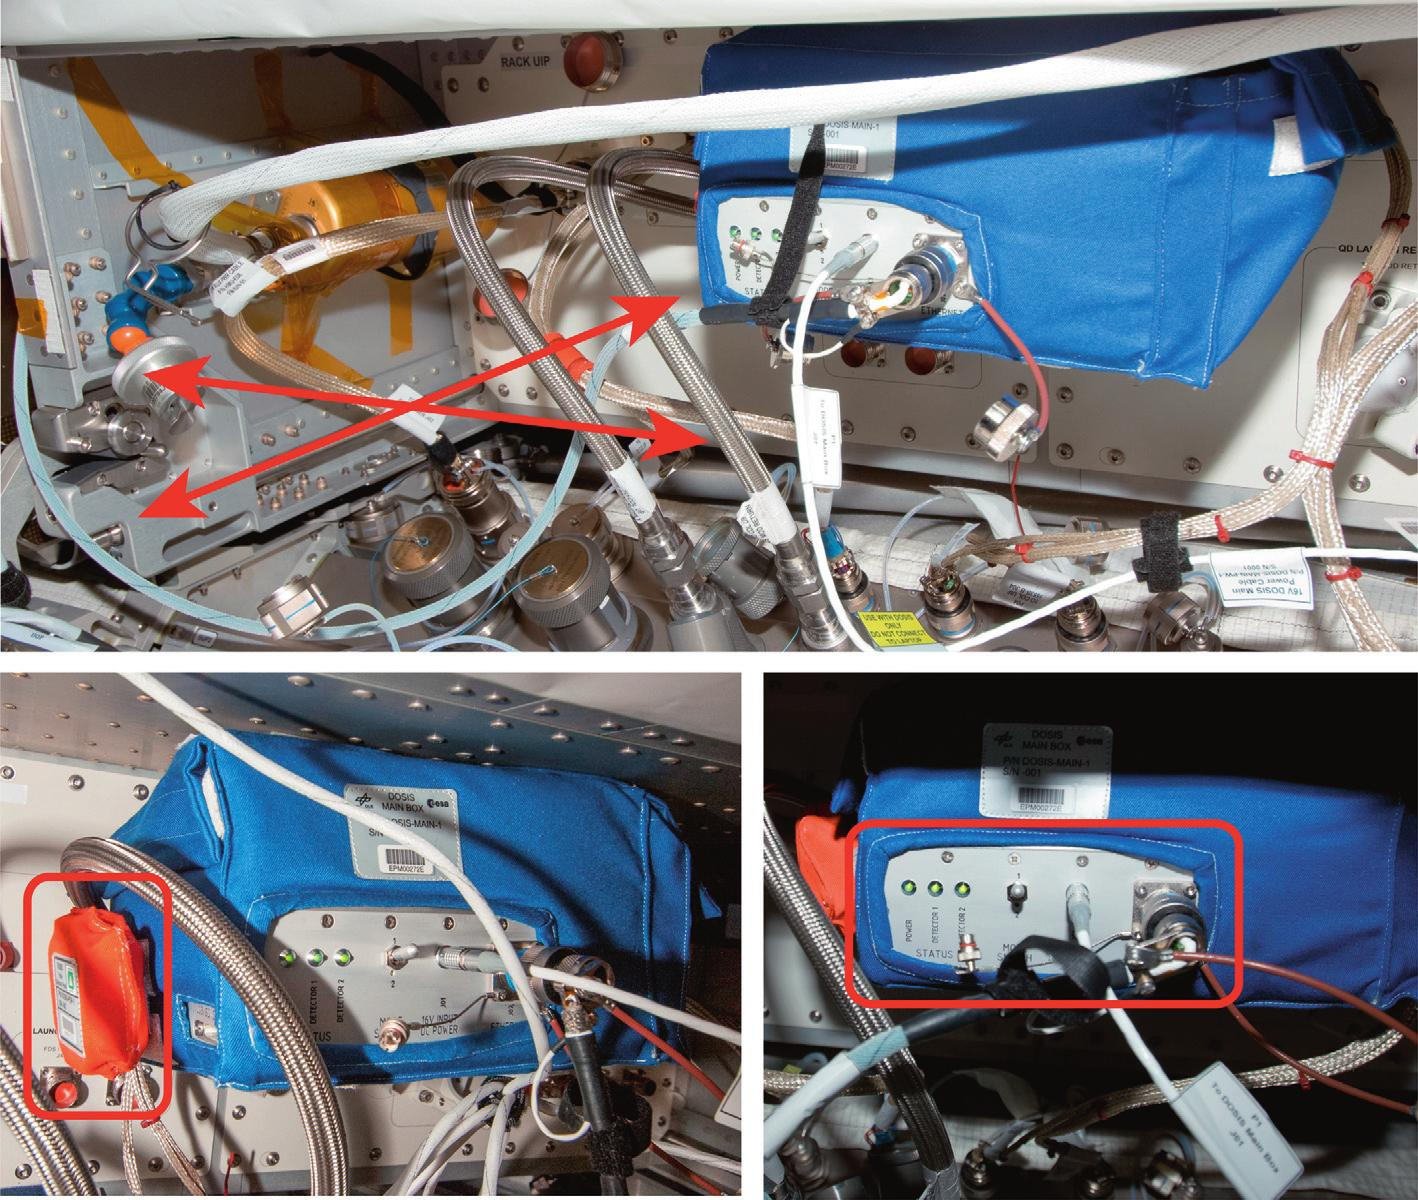
\includegraphics[width=0.8\textwidth]{dosis_activeDetectors.jpg}
  \caption{V horním obrázku je vidět modrý box, v němž jsou umístěny oba dva DOSTEL detektory; šipky ukazují namíření detektorů. Vlevo dole je vidět označený PDP připojený v blízkosti aktivních detektorů, vpravo dole je ukázáno ovládání jednoho DOSTELu. \cite{dosis2}}
  \label{fig:dosis_activeDetectors}
\end{figure}

%\subsection{Detektory používané NPI}
%NPI používá dva TL detektory, Al$_2$O$_3$:C a CaSO$_4$:Dy. Oba dva jsou vyhodnocovány pomocí čtecího systému RA’94 (THORN EMI 9789 QB)+TOLEDO 654 TLD Reader; rychlost zahřívání u obou je rovna 10 $^{\circ}$C/s; první není předehříván, druhý je předehříván na 150 $^{\circ}$C (22 s); annealing probíhá 20 minut za 700 $^{\circ}$C (Al$_2$O$_3$:C), respektive 10 minut za 380 $^{\circ}$C (CaSO$_4$:Dy); ochlazovací rychlost je vysoká u obou; kalibrování probíhá u obou pomocí $^{137}$Cs; u obou je vyhodnocována plocha pod vyhřívací křivkou. Oba dva mají průměr roven 5 mm a tloušťku rovnou 1 mm.


%Z TED používá NPI HARZLAS TD-1 a od roku 2016 i TASTRAK. HARZLAS TD-1 je leptán 18 hodin za teploty 70 $^{\circ}$C v 5 N koncentrovaném roztoku NaOH; odleptaná vrstva je kolem 15,3 $\mu$m. Většinou je analyzována plocha o velikosti 0,09 cm$^2$. Detektor je tlustý 0.9 mm. TASTRAK se leptá dvoufázově: první fáze trvá 6 hodin a jsou při ní zobrazeny stopy vytvořené částicemi s velkým $\mathit{LET}$; při druhé fázi, která trvá dalších 9 hodin, se zobrazí i stopy pocházejících od částic s nižším $\mathit{LET}$. Celkový čas leptání je tedy 15 hodin. Buď se postupuje postupným leptáním (6 hodin leptání, vyhodnocení, 9 hodin leptání, vyhodnocení), nebo se část detektoru leptá 6 hodin a část 15 hodin, tudíž
%detektor lze vyhodnotit najednou. Detektor se leptá při 70 $^{\circ}$C v 6,25 N koncentrovaném roztoku NaOH, odleptaná vrstva je tlustá 7,5/20,1 $\mu$m; analyzuje se plocha o velikosti 0,5 cm$^2$ (v obou případech) z důvodu zajištění dostatečné statistiky. Po leptání následuje u obou detektorů nasnímání stop lineárním snímacím zařízením s vysokým rozlišením (které je součástí mikroskopu HSP-1000, \cite{dosis_HSP1000}), poté jsou snímky se stopami analyzovány programem HspFit.

%To. že nám (NPI) vyšla kalibrační krivka jinak než těm madarum, tak to psat do casti o detektorech
\section{Data z luminiscenčních detektorů}\label{sec:dosis_vysledky}
Zde jsou uvedeny výsledky publikované v \cite{dosis}. Jedná se o data naměřená TL a OSL detektory z obou sad DOSIS a z prvních šesti sad DOSIS3D, tedy o data naměřená mezi lety 2009 a 2015. %Pro větší názornost jsou zde uvedeny i obrázky z \cite{dosis2}, které byly získány z dat naměřených aktivními detektory. 

Na naměřená data lze pohlížet z několika hledisek. Nejprve je uvedeno srovnání dat získaných z několika TL a ze všech OSL detektorů v rámci jedné sady experimentu DOSIS3D, konkrétně druhé. Poté následuje srovnání dat, které byly získány TL detektorem $^7$LiF:Mg,Ti v rámci všech osmi vyhodnocených sad. Dále je zmíněno stručné porovnání dat z pasivních a aktivních detektorů a nakonec jsou výsledky srovnány s daty získaných během jiných experimentů (popsaných ve článcích \cite{passDetectors, dataTLD_RR, ambrozova_dvaExperimenty, pille, pille2, wrmiss_SPD, japonsky}).
%Srovnáním dat od TL detektorů z DOSIS3D s daty získanými v ISS mimo modul Columbus od detektorů stejného materiálu plyne, že velmi závisí na lokálním stínění. Data se v závislosti na jeho tloušťce mohou lišit až dvojnásobně.  
%Vzhledem k tomu, že tato práce je primárně zaměřena na detektory stop v pevné fázi, tak jsou informace v tomto oddíle značně povrchní. %MOZNA ZMENIT?!!!!
\subsection{Srovnání dat pasivních detektorů v rámci jedné sady}
V obr. \ref{fig:dosis_vysl_jednaSada} jsou uvedeny dávkové příkony naměřené detektory z 2. sady DOSIS3D v závislosti na pozici detektoru, tzn. na PDP. Jedná se o TL detektory z materiálů: $^6$LiF:Mg,Ti; $^7$LiF:Mg,Ti; CaF$_2$:Tm; $^{\text{Nat}}$LiF:Mg,Ti; $^6$LiF:Mg,Cu,P; $^7$LiF:Mg,Cu,P; Al$_2$O$_3$:C a CaSO$_4$:Dy a o všechny OSL detektory. Je vidět, že data ze všech detektorů sledují v podstatě stejný trend a že dávkové příkony z detektorů stejného materiálu vycházejí přibližně stejně. Avšak na druhou stranu jsou zde patrné rozdíly mezi naměřenými dávkovými příkony detektorů různých materiálů. Jedním z důvodů je rozdílná účinnost detekce těžkých nabitých částic každého TL/OSL materiálu (viz oddíl \ref{sec:detektory_TLD}).
\begin{table}[H]
  \centering
  \def\arraystretch{0.8}
  \caption{Poměry odezev TLD materiálů s odezvou referenčního $^7$LiF:Mg,Ti. Odezvou se myslí určená dávka z daného detektoru \cite{dosis}.}
  \label{tab:dosis_TLD_ratio}
  \begin{tabular}{ll}
	\toprule
	Materiál & Poměr odezev\\
	\midrule
$^6$LiF:Mg,Ti		&1,06\\
$^{\text{Nat}}$LiF:Mg,Ti	&1,06\\
$^6$LiF:Mg,Cu,P		&0,90\\
$^7$LiF:Mg,Cu,P		&0,87\\
Al$_2$O$_3$:C (OSLD)&1,04\\ 
CaF$_2$:Tm			&1,01\\
CaSO$_4$:Dy			&0,88\\
Al$_2$O$_3$:C (TLD)	&0,82\\
\bottomrule
  \end{tabular}
\end{table}

Dávkový příkon od $^6$LiF:Mg,Ti, respektive $^6$LiF:Mg,Cu,P je systematicky vyšší než od $^7$LiF:Mg,Ti, resp. $^7$LiF:Mg,Cu,P, což je způsobeno tím, že nuklid $^6$Li má velký účinný průřez pro reakci ($n,\alpha$) s tepelnými neutrony. Nicméně rozdíl mezi těmito dvěma materiály není absorbovaná dávka pocházející od neutronů, ale od záření $\gamma$. Tato dávka je takové velikosti, aby vyvolala stejný termoluminiscenční signál jako skutečně obdržená dávka od neutronů. Tento jev je nazýván gamma ekvivalent neutronové dávky (``gamma-equivalent neutron dose''), \cite{dosis}.

V tab. \ref{tab:dosis_TLD_ratio} jsou poměry dávek určených výše zmíněnými detektory s dávkou určenou z TL materiálu $^7$LiF:Mg,Ti. Je vidět, že detektory od NPI mají nejmenší účinnost.

Výsledky z OSLD jsou celkem ve shodě vzhledem k rozmanitosti vyhodnocovacích metod.
\begin{figure}[!t]
  \centering
  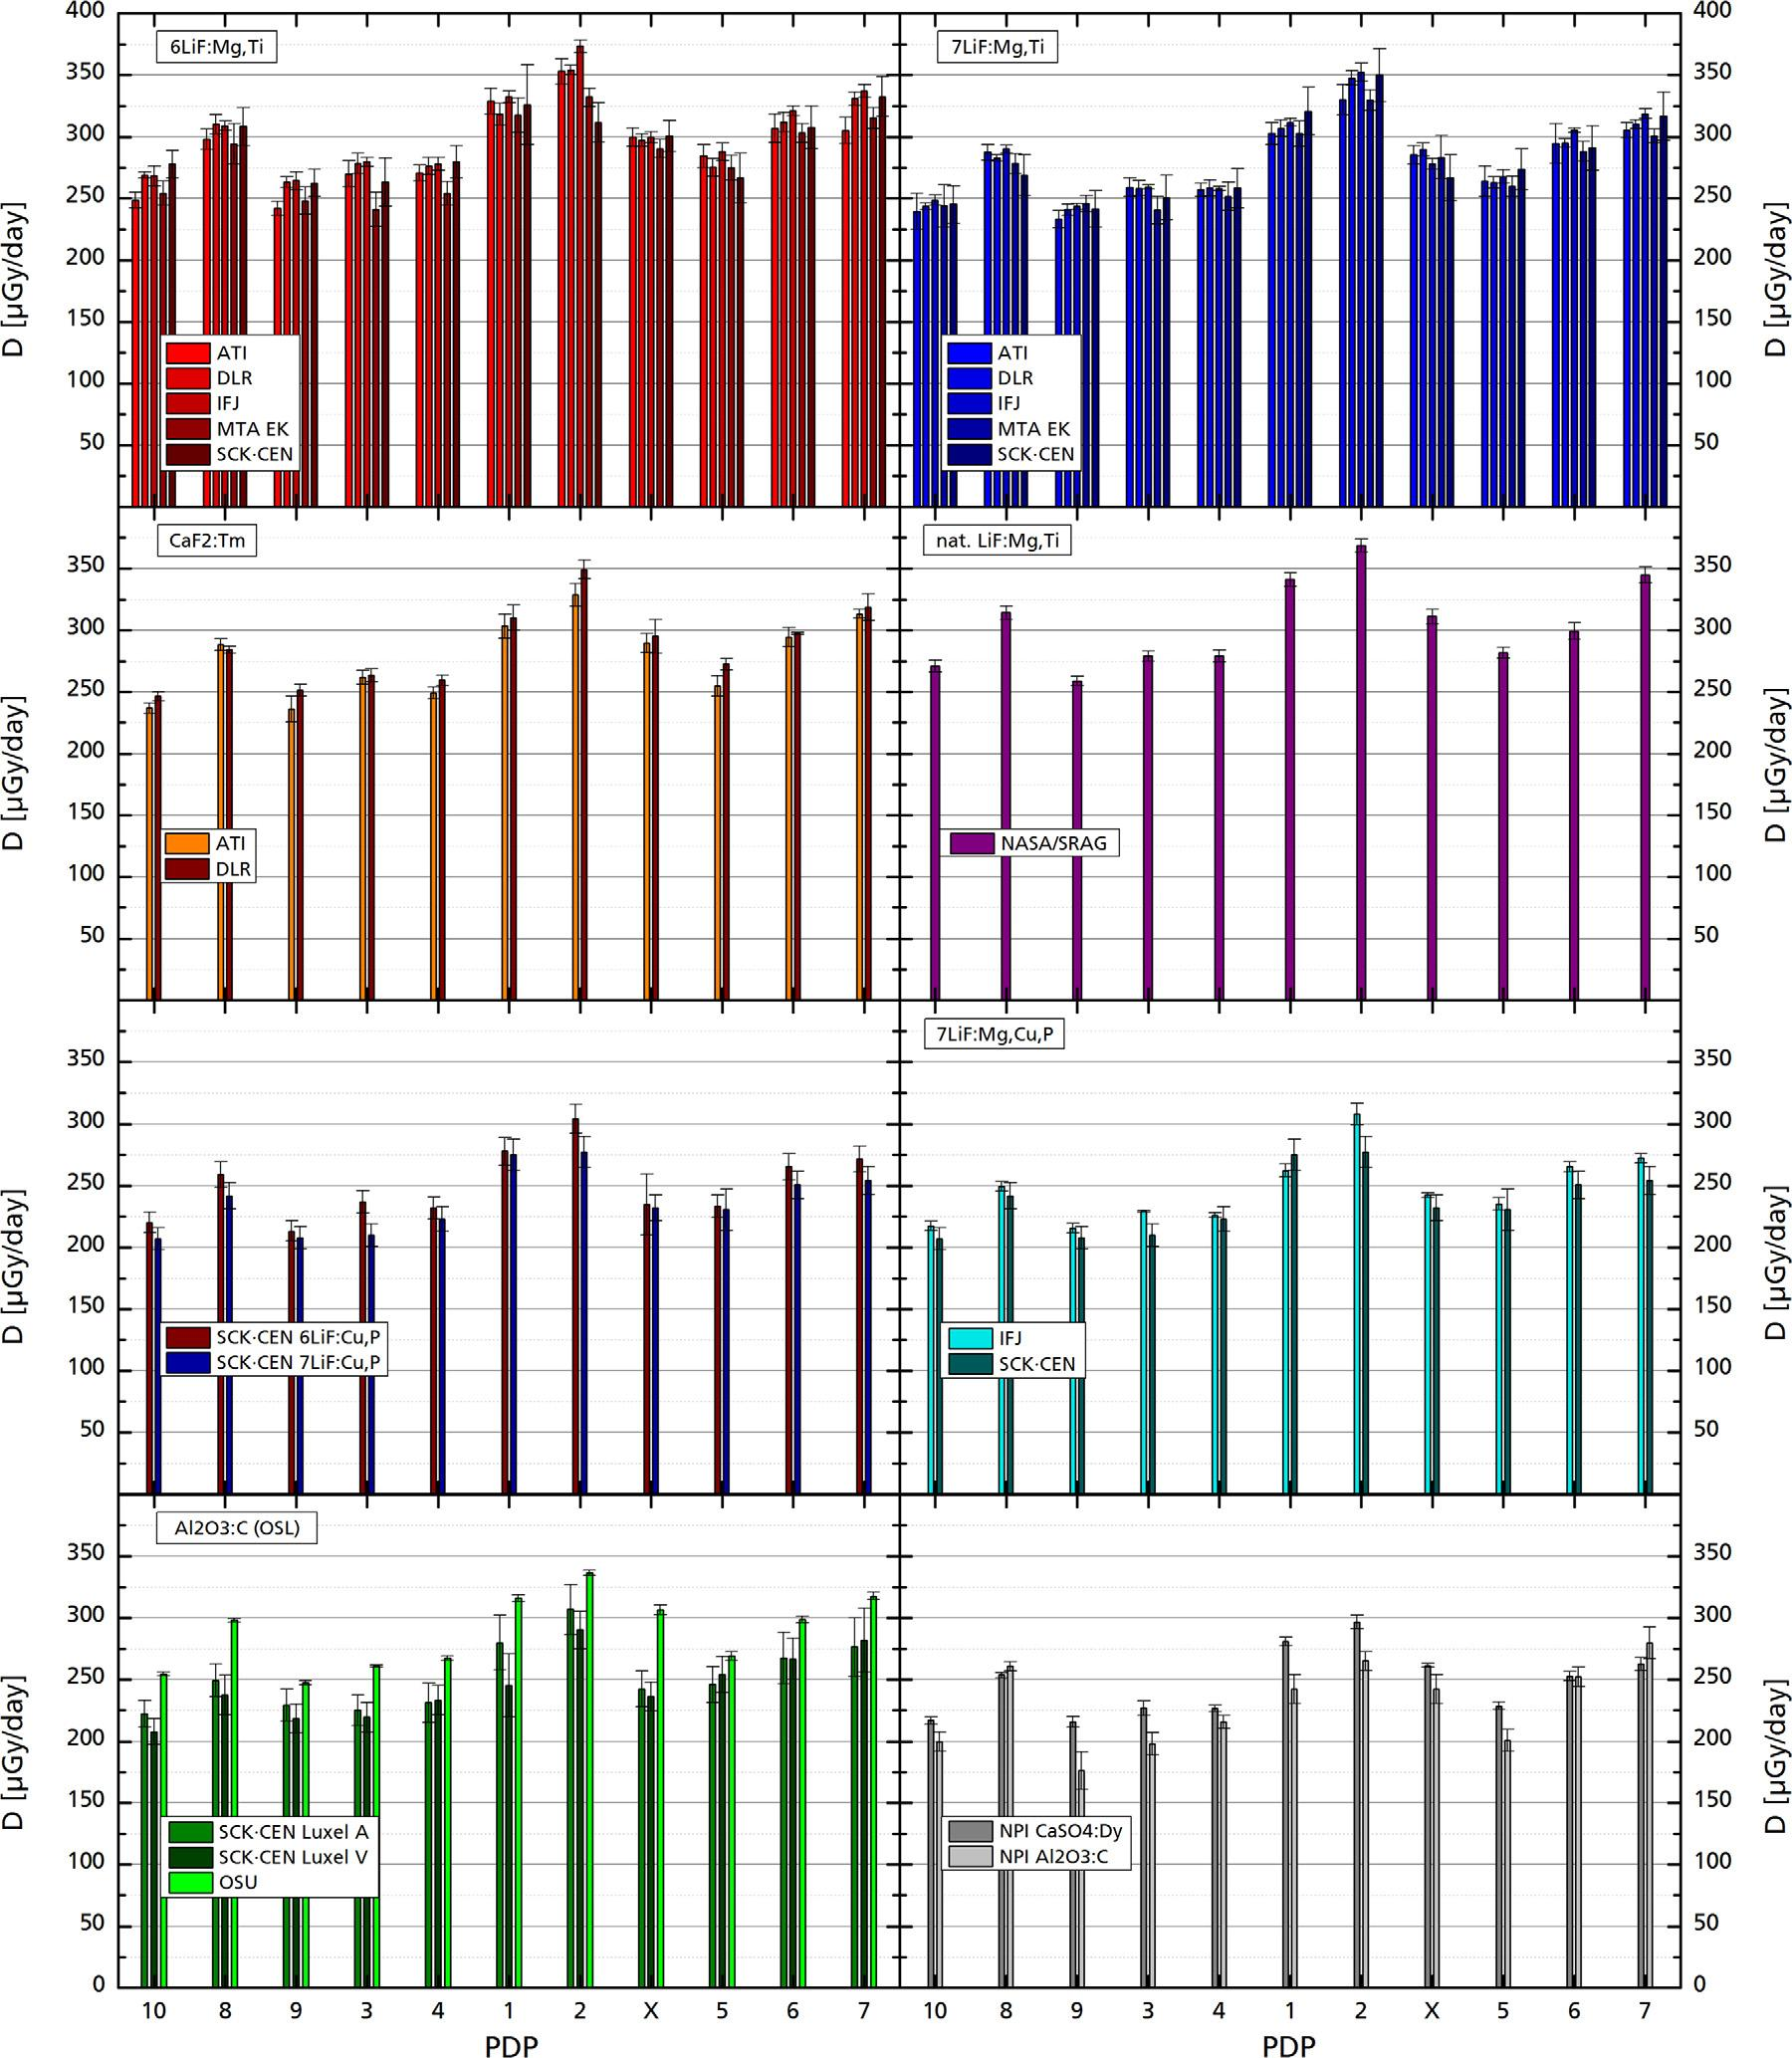
\includegraphics[height=0.65\textheight]{dosis_vysl_jednaSada.jpg}
  \caption{Naměřené dávkové příkony detektory různých materiálů. Na ose $x$ jsou čísla PDP, jejichž pořadí je založeno na poloze PDP v modulu Columbus (viz \ref{fig:columbus_rozmisteni}) \cite{dosis}.}
  \label{fig:dosis_vysl_jednaSada}
\end{figure}
\subsection{Srovnání dat z osmi sad pro jeden druh pasivního detektoru}
Srovnávala se data od TLD $^7$LiF:Mg,Ti ze všech PDP. Obr. \ref{fig:dosis_vysl_viceSad} zobrazuje zprůměrovaný rozsah dávkových příkonů ze všech PDP; průměrování probíhalo pro každé PDP jednotlivě přes příkony určené několika organizacemi.
%které byly určeny z dat $^7$LiF:Mg,Ti od několika organizací; 
Například pro D3D2 (druhá sada DOSIS3D) je interval naměřených dávkových příkonů přibližně [250, 350] $\mu$Gy/den (lze srovnat s obr. \ref{fig:dosis_vysl_jednaSada}). Na ose $x$ je čas v letech. Obrázek dále obsahuje v horní části nadmořskou výšku ISS a četnost neutronů naměřených Oulu monitorem (viz oddíl \ref{sec:dosis_altitudeSlunecniCyklus}). Pokles dávkového příkonu z DOS1 na DOS2 (sady 1 a 2 experimentu DOSIS) byl způsoben vzrůstající sluneční aktivitou; prudký vzrůst z DOS2 na D3D1 je spojen s nárazovitým zvýšením nadmořské výšky ISS; poté se už nadmořská výška moc neměnila a pomalý pokles je tedy dán
hlavně vzrůstající sluneční aktivitou. Je zajímavé, že při D3D6 detektory obdržely jen o trochu vyšší dávky než při DOS1.
\begin{figure}[h]
  \centering
  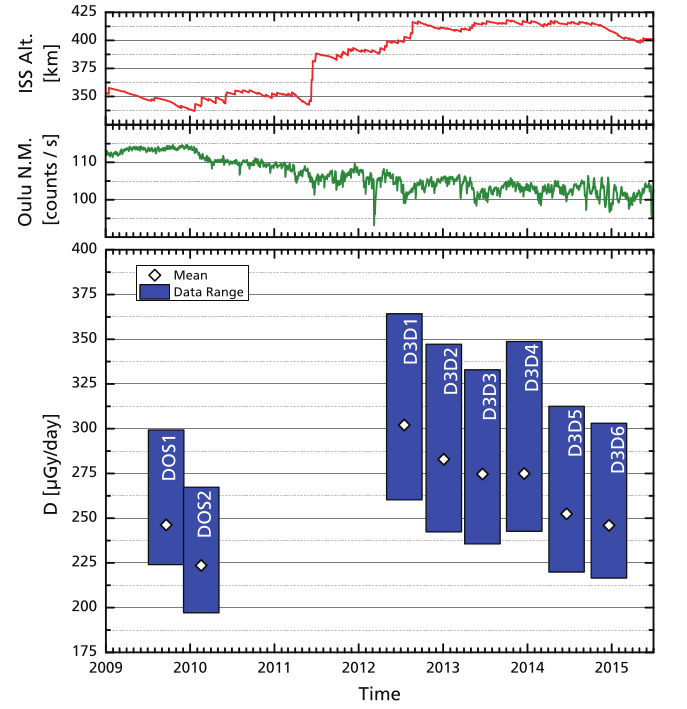
\includegraphics[width=0.65\textwidth]{dosis_vysl_viceSad.png}
  \caption{Rozsahy dávkových příkonů naměřených TLD materiálem $^7$LiF:Mg,Ti v rámci prvních osmi sad experimentů DOSIS a DOSIS3D. V horní části obrázku jsou parametry ovlivňující velikost obdržené dávky, tj. nadmořská výška ISS a četnost neutronů naměřená Oulu monitorem \cite{dosis_oulu}, která souvisí se sluneční aktivitou \cite{dosis}.}
  \label{fig:dosis_vysl_viceSad}
\end{figure}

U všech osmi sad sleduje dávkový příkon stejný vývoj přes 11 PDP jako v druhé sadě DOSIS3D (obr. \ref{fig:dosis_vysl_jednaSada}). Tento vývoj je  dán změnami v tloušťce lokálního stínění pro jednotlivé PDP, které velmi ovlivňují příspěvky od nízkoenergetických protonů při průletech nad SAA (viz oddíl \ref{sec:kosmickeZareni_stineni}). 

Absorbovaná dávka z detektorů, které byly umístěny u čelní stěny vzhledem k pohybu ISS (jedná se o PDP 3, 4, 8, 9, 10), je systematicky menší než absorbovaná dávka z detektorů umístěných u zadní stěny (PDP 1, 2, 5, 6, 7, X)~\cite{dosis}. To je možné vysvětlit anizotropií zachycených protonů v SAA (viz oddíl \ref{sec:kosmickeZareni_anizotropie}).
\subsection{Srovnání dat pasivních a aktivních detektorů}%řešit tu vodu (absorbed dose in water)???!!!!!!!!
V tab. \ref{tab:dosis_vysl_srovnaniPassiveActive} jsou srovnány dávkové příkony určené pomocí $^7$LiF:Mg,Ti a pomocí aktivního detektoru DOSTEL-1. Data od $^7$LiF:Mg,Ti pocházejí z PDP X (viz obr.~\ref{fig:columbus_rozmisteni}), který je upevněn na boxu, v němž se nachází aktivní detektory (viz obr.~\ref{fig:dosis_activeDetectors}). Absorbované dávky aktivního detektoru byly určeny zprůměrováním dat přes časový interval odpovídající dané sadě (viz tab. \ref{tab:dosis_timeline_passive}). Hodnoty v tab. \ref{tab:dosis_vysl_srovnaniPassiveActive} představují přepočtené absorbované dávky ve vodě. Je vidět, že data z obou typů detektorů jsou ve shodě. 

Při porovnávání dat z TLD a DOSTEL je třeba brát v úvahu několik věcí. Zaprvé účinnost detekce částic nad cca 10 keV/$\mu$m u TLD klesá, zatímco u DOSTEL je v podstatě stále stoprocentní. Dále pasivní detektory byly v PDP umístěny okolo 95~\% svého měřícího cyklu, zbytek času strávily cestováním na, resp. z ISS; nicméně toto pravděpodobně nezaneslo do měření nějakou větší chybu, protože při průletu atmosférou detektory obdrží zanedbatelnou dávku díky krátkému času letu.
\begin{table}[H]
  \centering
  \def\arraystretch{1}
  \footnotesize
  \caption{Porovnání dávkových příkonů určených pomocí aktivního detektoru DOSTEL-1 a pomocí TLD (materiál $^7$LiF:Mg,Ti), které byly umístěny v PDP X, v rámci dosud vyhodnocených sad~\cite{dosis}.}
  \label{tab:dosis_vysl_srovnaniPassiveActive}
  \begin{tabular}{lll|ll}
	\toprule
	&\multirow{2}{*}{Sada}&\multirow{2}{*}{Nadmořská výška ISS [km]}&\multicolumn{2}{c}{Absorbovaná dávka [$\mu$Gy/den]}\\
	 & & &DOSTEL-1&$^7$LiF:Mg,Ti\\
	\midrule
	DOSIS	&1&339-348&$248\pm20$&$261\pm21$\\ 
			&2&337-349&$234\pm18$&$238\pm10$\\
	DOSIS3D	&1&397-417&$286\pm25$&$311\pm9 $\\
			&2&407-416&$288\pm20$&$281\pm9 $\\
			&3&407-416&$297\pm23$&$294\pm7 $\\
			&4&413-418&$294\pm23$&$294\pm12$\\
			&5&413-417&$279\pm22$&$262\pm7 $\\
			&6&401-416&$256\pm20$&$256\pm7 $\\
	\bottomrule
  \end{tabular}
\end{table}

Výhodou aktivních detektorů je, že dokážou rozeznat příspěvky k dávce od GCR a od zachycených protonů v SAA.
\subsection{Srovnání s jinými experimenty}
\begin{itemize}
\item Na různých místech v americké části ISS jsou od organizace NASA/SRAG umístěné tzv. monitory prostorového rozložení záření (RAM, Radiation Area Monitor), které obsahují termoluminiscenční detektory ($^7$LiF:Mg,Ti) a slouží ke stanovení prostorové distribuce dávky v ISS~\cite{RAM}. Můžeme tedy srovnávat jejich výsledky s výsledky DOSIS/DOSIS3D. RAM detektory měřily na ISS od dubna 2014 do listopadu 2014, celkem 218 dní; tato doba pokrývá pátou a částečně i šestou sadu DOSIS3D (tab.~\ref{tab:dosis_timeline_passive}). V modulu Columbus byly naměřeny dávkové příkony v rozsahu $[216\pm8;313\pm9]$ $\mu$Gy/den, v rámci programu RAM bylo rozpětí naměřených dávkových příkonů $[201\pm5;421\pm12]$ $\mu$Gy/den. Minimum je tedy přibližně stejné, avšak maximum je vyšší pro RAM. To bylo naměřeno v
  blízkosti okénka, a tudíž ho lze spojit s nižším stíněním. Celkově lze z těchto srovnání tvrdit, že dávkové příkony se v jednotlivých modulech mohou v závislosti na lokálním stínění lišit až dvojnásobně.~\cite{dosis}

\item V letech 2007 a 2009 probíhalo měření spadající pod experiment MATROSHKA-R pomocí TLD (Al-P) a TED (HARZLAS TD-1, Page) v Ruském provozním modulu Zvezda (informace o modulu jsou k dohlednání např. v~\cite{serviceModule}) a v modulu Pirs~(\cite{piers1}); více o průběhu měření viz tab. \ref{tab:dosis_passDetectors_timeline}. Detektory byly v obou případech umístěny v šesti tzv. SPD (sborka passivnych detektorov, obdoba PDP u DOSIS\&DOSIS3D), přičemž dva SPD se nacházely v Pirs modulu a čtyři ve Zvezdě. 
\begin{table}[h]
  \centering
  \caption{Časový vývoj měření v ruských modulech Zvezda a Pirs. \cite{passDetectors}}
  \label{tab:dosis_passDetectors_timeline}
  \begin{tabular}{llll}
	\toprule
	Fáze&Počátek-konec&Doba trvání [dny]&Nadmořská výška ISS [km]\\
	\midrule
	1&Květen-Říjen 2007&163&338-353\\
	2&Květen-Říjen 2009&158&350-361\\
	\bottomrule
  \end{tabular}
\end{table}
Srovnejme nyní data od TLD Al-P z druhé fáze experimentu MATROSHKA-R (viz tab. \ref{tab:dosis_passDetectors_vysledky}) s daty od TLD $^7$LiF:Mg,Ti z první sady projektu DOSIS, která byla nainstalována v modulu Columbus od července 2009 do listopadu 2009 (dávkové příkony přibližně v rozmezí od 225 do 300 $\mu$Gy/den, viz obr. \ref{fig:dosis_vysl_viceSad}). 
\begin{table}[h]
  \centering
  \caption{Naměřené dávkové příkony TL detektorem Al-P při druhé fázi experimentu MATROSHKA-R v roce 2009. První dva SPD byly umístěny v modulu Pirs, ostatní ve Zvezdě. \cite{passDetectors}}
  \label{tab:dosis_passDetectors_vysledky}
  \begin{tabular}{lll}
	\toprule
	SPD&$\dot{D}$ [$\mu$Gy/den]\\
	\midrule
	1&$445\pm31$\\
	2&$417\pm29$\\
	3&$368\pm26$\\
	4&$387\pm27$\\
	5&$321\pm22$\\
	6&$301\pm21$\\
	\bottomrule
  \end{tabular}
\end{table}
Dávkové příkony z modulu Pirs jsou jasně nejvyšší, poté následují dávkové příkony z modulu Zvezda; horní hranice rozsahu dávkových příkonů z modulu Columbus odpovídá minimální hodnotě naměřené ve Zvezdě. Rozdíl mezi Pirsem a Zvezdou je dán rozdílem v tloušťce stínění \cite{passDetectors}. Stínění mohlo hrát roli i v naměření mnohem nižší dávky v modulu Columbus, avšak vzhledem k rozdílné relativní účinnosti Al-P a $^7$LiF:Mg,Ti to nemůžeme tvrdit. Na obr. \ref{fig:dosis_passDetectors_LETspektrum} jsou srovnána $\LET$ spektra z modulu Pirs (SPD 2) a z modulu Zvezda (SPD 6); je zcela jasně vidět, že méně stíněný Pirs obdržel větší dávku od částic s $\LET<100$ keV/$\mu$m, u částic s vyšším $\LET$ žádný rozdíl
není \cite{passDetectors}. (Poznámka: lze srovnat obr. \ref{fig:dosis_passDetectors_LETspektrum} s obr. \ref{fig:stineni} -- rozdíl ve spektrech je způsoben tím, že první obr. představuje diferenciální spektrum, zatímco druhý zobrazuje integrální spektrum.) 
\begin{figure}[h]
  \centering
  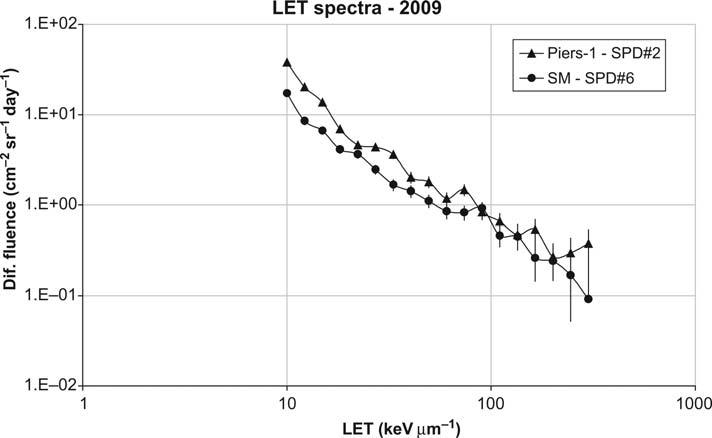
\includegraphics[width=0.65\textwidth]{dosis_LETspektrum_passDetectors.jpg}
  \caption{$\LET$ spektra z dat naměřených v modulu Pirs (Piers-1) a v modulu Zvezda (SM) v příslušných SPD.~\cite{passDetectors}}
  \label{fig:dosis_passDetectors_LETspektrum}
\end{figure}
\item Lepší srovnání poskytuje měření z roku 2012, které také proběhlo v rámci MATROSHKA-R. Bylo prováděno TL detektorem CaSO$_4$:Dy, který byl umístěn na šesti pozicích v ruské části ISS (jeden byl v modulu Pirs, jeden v ruském výzkumném modulu~\cite{researchModule} a čtyři v modulu Zvezda). Měření započalo v květnu 2012 a probíhalo jeden rok, což odpovídá první a druhé sadě experimentu DOSIS3D. Průměrný dávkový příkon naměřený ve Zvezdě je roven 262 $\mu$Gy/den, což je velmi blízké hodnotě průměrného dávkového příkonu naměřeného v rámci DOSIS3D (TL detektorem CaSO$_4$:Dy), který je roven 275 $\mu$Gy/den. Data z Pirsu a výzkumného modulu dosahují hodnot okolo 500 $\mu$Gy/den, jedná se zase o důsledek nižšího stínění. Z uvedených informací (i z předchozích odrážek) plyne, že za předpokladu
  stálosti nadmořské výšky a dalších parametrů jsou rozdíly v dávkách dány hlavně stíněním celého objektu, menší rozdíly jsou pak způsobeny lokálním stíněním (které je představováno např. uloženými zásobami, přístroji).~\cite{ambrozova_dvaExperimenty}
  \item Článek~\cite{ambrozova_dvaExperimenty} poskytuje i porovnání s daty, které byly naměřeny v jiné nadmořské výšce. Satelit BION-M1 byl vypuštěn 19. dubna 2013 a na orbitě o nadmořské výšce 575 km setrval 30 dní. Obsahoval mj. biologické vzorky a detektory, konkrétně TLD CaSO$_4$:Dy a TED HARZLAS TD-1. Ty byly uloženy ve čtyřech boxech uvnitř satelitu a ve dvou boxech na vnějším plášti satelitu. Průměr z dávkových příkonů naměřených ve vnitřních boxech pomocí TLD činí 967 $\mu$Gy/den, ve vnějších boxech 2,2 mGy/den. Nadmořská výška ISS byla přibližně 409 km a v modulu Columbus byl naměřen dávkový dávka cca 275 $\mu$Gy/den, viz předchozí odrážka. Tyto obrovské rozdíly v naměřených hodnotách ukazují důležitost vlivu změny nadmořské výšky (ISS proti BION-M1, ovšem dále je třeba vzít v úvahu, že BION-M1 měl méně
	stíněn) a stínění (vnitřek proti vnějšku satelitu BION-M1).
  \item V japonském modulu Kibo \cite{kibo} probíhá již od jeho připojení k ISS v roce 2008 měření pomocí TLD (prášek Mg$_2$SiO$_4$:Tb) a TED (CR-39 materiály HARZLAS TD-1 a Fukuvi chemical) v rámci projektu PADLES (PAssive Dosimeters for Lifescience Experiments in Space). V letech 2008 až 2010 proběhly tři obměny detektorů (viz tab.~\ref{tab:dosis_kibo}).
	\begin{table}[ht]
	  \centering
	  \caption{Obměna PADLES v modulu Kibo. \cite{japonsky}}
	  \label{tab:dosis_kibo}
	  \begin{tabular}{llll}
		\toprule
	Fáze&Počátek-konec&Doba trvání [dny]&Nadmořská výška ISS [km]\\
	\midrule
	1&Červen 2008-Březen 2009&278&339-359\\
	2&Březen 2009-Srpen 2009&164&343-355\\
	3&Září 2009-Duben 2010&214&337-350\\
	\bottomrule
	  \end{tabular}
	\end{table}
	Detektory byly umístěny na dvanácti pozicích v Přetlakovém modulu, v případě třetí fáze navíc i na pěti pozicích v Logistickém modulu (přetlaková komora). Průměrný dávkový příkon naměřený TLD v první fázi je $311\pm 30$ $\mu$Gy/den, v druhé fázi $268\pm29$ $\mu$Gy/den, v třetí fázi pro Přetlakový modul $286\pm33$ $\mu$Gy/den a pro Logistický modul $289\pm27$ $\mu$Gy/den. V době první fáze PADLES experiment DOSIS ještě neprobíhal. Druhá a třetí fáze PADLES odpovídá přibližně první a druhé sadě experimentu DOSIS (červenec 2009 až květen 2010). Rozsahy dávkových příkonů z $^7$LiF:Mg,Ti z těchto sad jsou přibližně $[225;300]$ $\mu$Gy/den, resp. $[200;265]$ $\mu$Gy/den (viz obr. \ref{fig:dosis_vysl_viceSad}). Vidíme, že data z modulů Kibo a Columbus jsou velmi podobná. To, že $\dot{D}$ z druhé fáze na třetí fázi PADLES
	vzrostl,
	zatímco u DOSIS klesl, může být dáno různým počátkem a koncem fází u PADLES a DOSIS. \cite{japonsky}
  \item K monitorování dávkových příkonů v ISS se používá i Pille TLD systém. Tento systém byl využíván na každé kosmické stanice od druhé poloviny 70. let 20. století.
	\begin{table}[ht]
	  \centering
	  \caption{Rozsahy průměrných týdenních dávkových příkonů naměřených TLD systémem Pille v daný časový úsek~\cite{pille, pille2}. Za dvojitou svislou čárou jsou průměrné dávkové příkony od CaSO$_4$:Dy pro $i$-tou sadu DOSIS3D, kde $i=$číslo řádku.}
	  \label{tab:dosis_pille}
	  \begin{tabular}{l|l||l}
		\toprule
		\multicolumn{2}{c||}{Pille-Zvezda}&DOSIS3D\\
		\midrule
		Časový úsek&$\dot{D}$ [$\mu$Gy/den]&$\dot{D}$ [$\mu$Gy/den]\\
		\midrule
		Květen $\ $ 2012-Říjen 2012&$[160;200]$&$264$	\\
		Listopad 2012-Duben  2013&$[150;210]$&$250$	\\
		Květen $\ $ 2013-Listopad 2013&$[165;190]$&$240$	\\
		Listopad 2013-Květen  2014&$[140;180]$&$240$	\\
		Květen $\ $ 2014-Listopad 2014&$[140;170]$&$220$	\\
		Listopad 2014-Březen  2015&$[130;160]$&$215$	\\
		\bottomrule
	  \end{tabular}
	\end{table}
	 Jedná se o TL detektor CaSO$_4$:Dy (avšak v jiné formě než v jakou používá NPI) s čtecím systémem, což umožňuje vyhodnocovat detektory přímo na orbitě. Na ISS se nachází v modulu Zvezda od roku 2003, kde se používá jako osobní dozimetr při CME, při výstupech do vesmíru a také pro mapování prostorové distribuce dávky. Detektory byly v roce 2009 obměněny a v současnosti se jich ve Zvezdě nachází dvanáct. Naměřené dávky neprošly korekcí na $\LET_{\text{H$_2$O}}>10$ keV/$\mu$m a nebyly převedeny na absorbované dávky ve vodě (resp. tkáňově ekvivalentním materiálu). V levé části tab. \ref{tab:dosis_pille} jsou
	 přibližné rozsahy průměrných týdenních dávkových příkonů naměřených v daný časový úsek.	První časový úsek Pille odpovídá přibližně první sadě DOSIS3D, druhý úsek druhé sadě DOSIS3D a takto to pokračuje až k šestému úseku/šesté sadě. Pravá část tab.~\ref{tab:dosis_pille} obsahuje průměrné hodnoty dávkových příkonů od CaSO$_4$ pro danou sadu; tyto dávkové příkony byly získány přenásobením průměrné hodnoty z $^7$LiF:Mg,Ti (viz obr.~\ref{fig:dosis_vysl_viceSad}) poměrem odezev CaSO$_4$:Dy a $^7$LiF:Mg,Ti (viz tab.~\ref{tab:dosis_TLD_ratio}). Vidíme, že dávkové příkony od Pille jsou systematicky nižší. Částečně to bude dáno tím, že výsledky od Pille nejsou převedeny na absorbovanou dávku ve vodě. Dále pozorujeme, že $\dot{D}$ od Pille sleduje podobný trend jako
	 $\dot{D}$ od DOSIS3D, tzn. pozvolné klesání.~\cite{pille, pille2}
 \end{itemize}
 \textbf{Shrnutí:} V první odrážce jsme srovnali $\dot{D}$ z DOSIS\%DOSIS3D s $\dot{D}$ z americké části ISS (program RAM). Dávkové příkony z RAM měly stejnou minimální hodnotu jako dáv. příkony z modulu Columbus, ale maximální hodnotu měly vyšší. Také se zjistilo, že dávkové příkony se mohou lišit v jednom modulu v závislosti na lokálním stínění až dvojnásobně.
 
 Ve druhé, třetí a šesté odrážce jsme data z DOSIS\&DOSIS3D srovnávali s daty naměřenými v ruské části ISS, hlavně v modulu Zvezda. V druhé odrážce jsme zjistili, že dávkové příkony byly vyšší ve Zvezdě, naopak v třetí a páté vyšly dávkové příkony vyšší v modulu Columbus. Příčinou jiného výsledku v druhé odrážce jsou pravděpodobně odlišné relativní účinnosti použitých TLD (experimentů diskutovaných v druhé odrážce).

 V páté odrážce jsme porovnali dávkové příkony z modulu Columbus s dávkovými příkony v japonském modulu Kibo. Dávkové příkony vycházejí podobně.

 Ve čtvrté odrážce proběhlo srovnání s dávkovými příkony naměřenými v satelitu BION-M1, který měl cca o 170 km větší nadmořskou výšku než ISS. To korelovalo s mnohem vyššími dávkovými příkony oproti $\dot{D}$ z modulu Columbus. Dávkové příkony z povrchu pláště satelitu jsou více jak dvojnásobné ve srovnání s dávkovými příkony uvnitř satelitu.


 %Srovnáním dat od TL detektorů z DOSIS3D s daty získanými v ISS mimo modul Columbus od detektorů stejného materiálu plyne, že velmi závisí na lokálním stínění. Data se v závislosti na jeho tloušťce mohou lišit až dvojnásobně.  

